 \ifx\PREAMBLE\undefined
\documentclass{report}
\usepackage[format = hang, font = bf]{caption}
\usepackage{subcaption}
% The following is needed in order to make the code compatible
% with both latex/dvips and pdflatex. Added for using UML generated by MetaUML.
\ifx\pdftexversion\undefined
\usepackage[dvips]{graphicx}
\else
\usepackage[pdftex]{graphicx}
\DeclareGraphicsRule{*}{mps}{*}{}
\fi
\usepackage{array}
\usepackage{amsmath}
\usepackage{amsthm}
\usepackage{mathtools}
\usepackage{boxedminipage}
\usepackage{listings}
\usepackage{multicol}
\usepackage{makecell}%diagonal line in table
\usepackage{float}%allowing forceful figure[H]
\usepackage{xcolor}
\usepackage{mathrsfs}%mathcal
\usepackage{amsfonts}%allowing \mathbb{R}
\usepackage{amssymb}
\usepackage{alltt}
\usepackage{algorithmicx}
\usepackage[chapter]{algorithm} 
%chapter option ensures that algorithms are numbered within each chapter rather than in the whole article
\usepackage[noend]{algpseudocode} %If end if, end procdeure, etc is expected to appear, remove the noend option
\usepackage{xspace}
\usepackage{physics}
\usepackage{color}
\usepackage{tikz}
\usetikzlibrary{shapes,positioning}
\usepackage{url}
\def\UrlBreaks{\do\A\do\B\do\C\do\D\do\E\do\F\do\G\do\H\do\I\do\J\do\K\do\L\do\M\do\N\do\O\do\P\do\Q\do\R\do\S\do\T\do\U\do\V\do\W\do\X\do\Y\do\Z\do\[\do\\\do\]\do\^\do\_\do\`\do\a\do\b\do\c\do\d\do\e\do\f\do\g\do\h\do\i\do\j\do\k\do\l\do\m\do\n\do\o\do\p\do\q\do\r\do\s\do\t\do\u\do\v\do\w\do\x\do\y\do\z\do\0\do\1\do\2\do\3\do\4\do\5\do\6\do\7\do\8\do\9\do\.\do\@\do\\\do\/\do\!\do\_\do\|\do\;\do\>\do\]\do\)\do\,\do\?\do\'\do+\do\=\do\#\do\-}
\usepackage{xr}%allow cross-file references
\usepackage[breaklinks = true]{hyperref}
\usepackage{thmtools}
\lstset{
language = C++, 
showspaces = false,
breaklines = true, 
tabsize = 2, 
numbers = left, 
extendedchars = false, 
basicstyle = {\ttfamily \footnotesize}, 
keywordstyle=\color{blue!70}, 
commentstyle=\color{gray}, 
frame=shadowbox, 
rulesepcolor=\color{red!20!green!20!blue!20}, 
numberstyle={\color[RGB]{0,192,192}}, 
moredelim=[is][\underbar]{_}{_}
}
\mathchardef\myhyphen="2D
% switch-case environment definitions
\algblock{switch}{endswitch} 
\algblock{case}{endcase}
%\algrenewtext{endswitch}{\textbf{end switch}} %If end switch is expected to appear, uncomment this line.
\algtext*{endswitch} % Make end switch disappear
\algtext*{endcase}
\algnewcommand\algorithmicinput{\textbf{Input}}
\algnewcommand\Input{\item[\algorithmicinput]}
\algnewcommand\algorithmicoutput{\textbf{Output}}
\algnewcommand\Output{\item[\algorithmicoutput]}
\algnewcommand\algorithmicinputoutput{\textbf{input and output:}}
\algnewcommand\InputOutput{\item[\algorithmicinputoutput]}
\allowdisplaybreaks
\newtheorem{theorem}{Theorem}
\newtheorem{corollary}[theorem]{Corollary}
\newtheorem{lemma}[theorem]{Lemma}
\newtheorem{definition}{Definition}
\renewcommand{\listtheoremname}{List of Important Theorems}
\begin{document}
\fi
\chapter{Block Ciphers}
\section{Overview}
Block cipher is a more powerful primitive than stream cipher. As with stream cipher, a block cipher is made up of an encryption algorithm $E$ and a decryption algorithm $D$, both of which take as input a key $k$. Both algorithms take as input $n$ bits, and output $n$ bits. There are two canonical examples of block ciphers:
\begin{description}
\item[3DES]$n$ = 64, $k$ = 168;
\item[AES]$n$ = 128, $k$ = 128/192/256.
\end{description}
A block cipher first expands the key $k$ into $t$ \textbf{round keys} $k_1,\dots,k_t$. Then it uses a \textbf{round function} $R(k,m)$ to encrypt the message by sequentially using the round keys and the encryption result in the previous step: $m_1=R(k_1,m),m_2=R(k_2,m_1),\dots,c=R(k_t,m_{t-1})$. We have $t=48$ for 3DES and $t=10$ for AES-128.

Typically block ciphers are slower than stream ciphers. But block ciphers are capable of completing some tasks that cannot be done efficiently with stream ciphers.

\begin{definition}\textbf{(PRF)}
A \textbf{pseudo random function (PRF)} is a function defined over $(K,X,Y)$:
\[F:K\times X\rightarrow Y\]
such that there exists an  \textbf{efficient} algorithm to evaluate $F(k,x)$. 
\end{definition}
\begin{definition}\textbf{(PRP)}
A \textbf{pseudo random permutation (PRP)} is a function defined over $(K,X,X)$:
\[E:K\times X\rightarrow X\]
such that 
\begin{itemize}
\item There exists an \textbf{efficient} deterministic algorithm to evaluate $E(k,x)$;
\item The function $E(k,\cdot)$ is one-to-one, i.e. it's invertible;
\item There exists an \textbf{efficient} inversion algorithm $D(k,y)$.
\end{itemize}
\end{definition}

A PRP is a PRF in which $X=Y$ and $F$ is efficiently invertible once $k$ is fixed. PRP captures accurately and syntactically what a block cipher is. AES is a PRP defined on
$K=X=\{0,1\}^{128}$. 3DES is a PRP defined on $K=\{0,1\}^{168}, X=\{0,1\}^{64}$. 

Let $F:K\times X\rightarrow Y$ be a PRF. Let $Funs[X,Y]$ represent the set of all functions from $X$ to $Y$ ($card(Funs[X,Y])=\lvert Y\rvert^{\lvert X\rvert}$), and $S_F$ represent the set of $F(k,\cdot)$ with $k\in K$($card(S_F)=card(K)$). Obviously $S_F\subseteq Funs[X,Y]$.
\begin{definition}\textbf{(Secure PRFs)}
We call $F$ a \textbf{secure PRF} if a random function from $Funs[X,Y]$ is indistinguishable from a random function from $S_F$.
\end{definition}
From a secure PRF $F:K\times \{0,1\}^n\rightarrow\{0,1\}^n$, we can easily construct a secure PRG $G:K\times\{0,1\}^{nt}$:
\[G(k)=F(k,0)\parallel F(k,1)\parallel\dots\parallel F(k,t).\]
A great property of this PRG is that it is computationally parallelizable. We will prove its correctness later.
\section{Data Encryption Standard (DES)}
In order to specify a block cipher, we need to provide the key expansion mechanism and the round function. DES will be used as an example in this section.
\subsection{Feistel Network}
The core idea behind DES is \textbf{Feistel network}. Its goal is to build an invertible function $F:\{0,1\}^{2n}\rightarrow\{0,1\}^{2n}$ from $n$ arbitrary (not necessarily invertible!) functions $f_1,f_2,\dots,f_d:\{0,1\}^n\rightarrow\{0,1\}^n$. The initial input contains two parts $R_0$ and $L_0$, each $n$ bits. Then we have 
\begin{equation*}\begin{cases}
R_i&=L_{i-1}\oplus f_i(R_{i-1})\\
L_i&=R_{i-1}
\end{cases}\end{equation*}
for $i=1,2,\dots,d$, as shown in Figure \ref{feistel}. $R_d,L_d$ are taken as the output. 
\begin{figure}[ht]
\centering
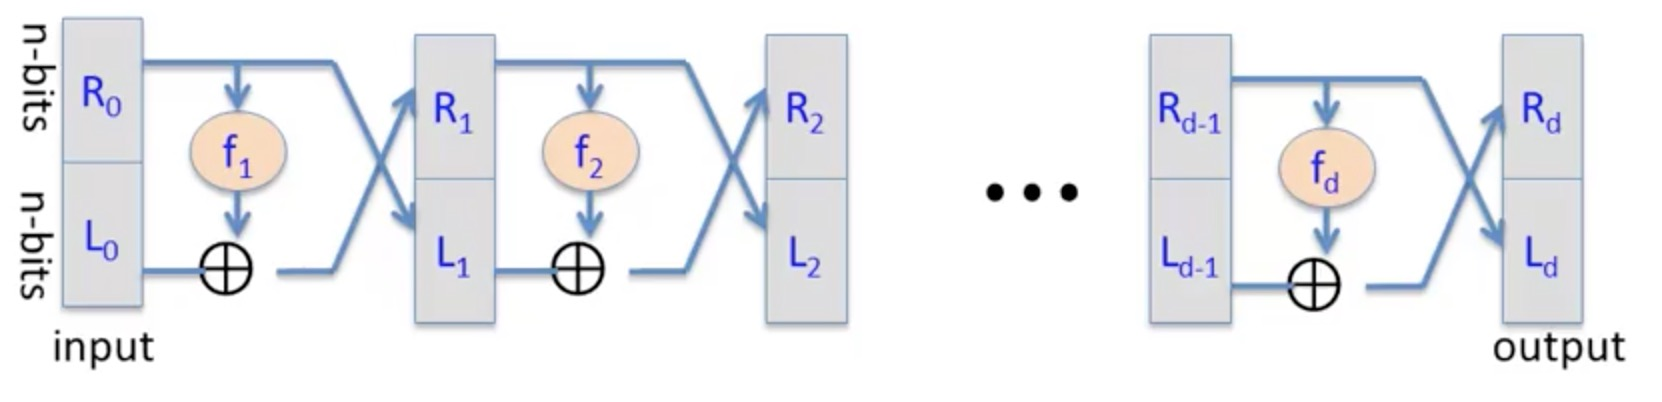
\includegraphics[width=\textwidth]{feistel.jpg}
\caption{Feistel Network}\label{feistel}
\end{figure}

It is easy to construct its inverse:
\begin{equation*}\begin{cases}
R_{i-1}&=L_i\\
L_{i-1}&=f_i(L_i)\oplus R_i
\end{cases}\end{equation*}
for $i=d,\dots,1$. Feistel network is used in many block ciphers, but not in AES.

The following theorem is important in the theory of DES. 
\begin{theorem}(Luby-Rackoff)\label{lubyrackoff}
If $f:K\times\{0,1\}^n\rightarrow\{0,1\}^n$ is a secure PRF, then a 3-round Feistel Network (Figure \ref{3rfeistel}) $F:K^3\times\{0,1\}^{2n}\rightarrow\{0,1\}^{2n}$ is a secure PRP.
\end{theorem}
\begin{figure}[ht]
\centering
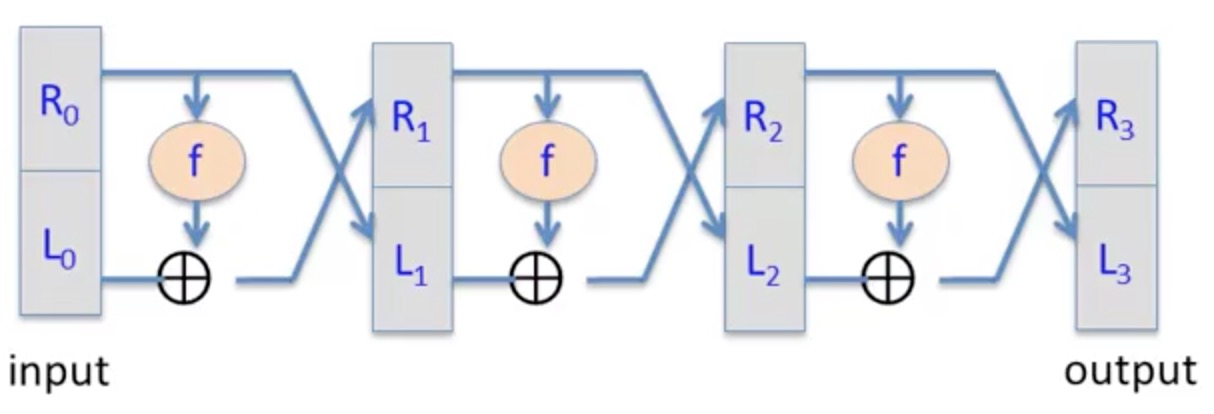
\includegraphics[width=\textwidth]{3rfeistel.jpg}
\caption{3-Round Feistel Network}\label{3rfeistel}
\end{figure}
The theorem means that if we have a secure PRF at hand, we can construct a secure block cipher.

DES is essentially a 16-round Feistel network. It uses 16 functions $F(k_i,x)=f_i(x):\{0,1\}^{32}\rightarrow\{0,1\}^{32},i=1,\dots,16$, as shown in Figure \ref{des}. IP is an initial permutator not for security reason, but required by the standard, and IP$^{-1}$ is its inverse. The Feistel network uses 16 48-bit keys expanded from a 56-bit initial key\footnote{We won't discuss the key expansion.}.
\begin{figure}[ht]
\centering
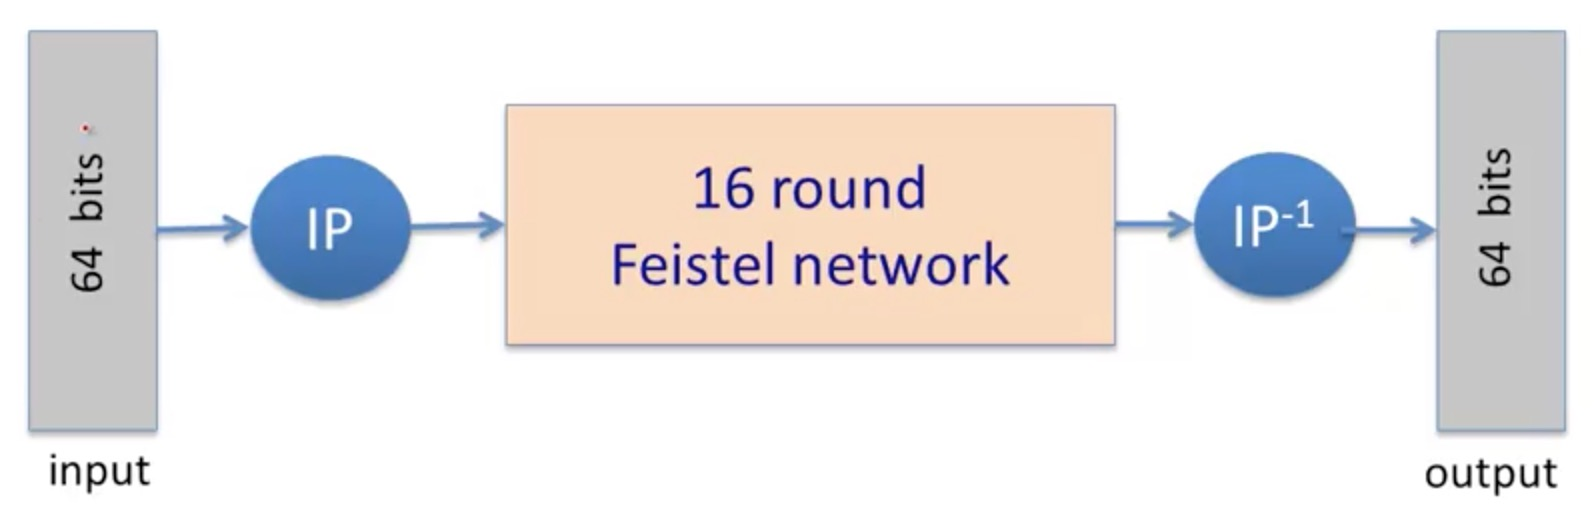
\includegraphics[width=\textwidth]{DES.jpg}
\caption{DES}\label{des}
\end{figure}
\subsection{DES Round Function}
Let's now discuss the round function $F(k_i,x)$. It carries out the following steps.
\begin{enumerate}
\item Pass the 32-bit input $x$ to an expansion box $E$, which expands it to 48 bits $x'$ by simply replicating and moving bits (i.e. linear operation that can be represented by a matrix)
\item Compute $x'\oplus k_i$ ($k_i$ is also 48 bits).
\item Break $x'\oplus k_i$ into 8 6-bit groups.
\item Each 6-bit group goes through an $S$ box and gets mapped to 4 bits.
\item Gather the 8 4-bit results and use a $P$ box to permute them into a 32-bit output.  
\end{enumerate}

The $S$ boxes are $\{0,1\}^6\rightarrow\{0,1\}^4$ functions implemented as lookup tables. Figure \ref{sboxeg} is an example.
\begin{figure}[ht]
\centering
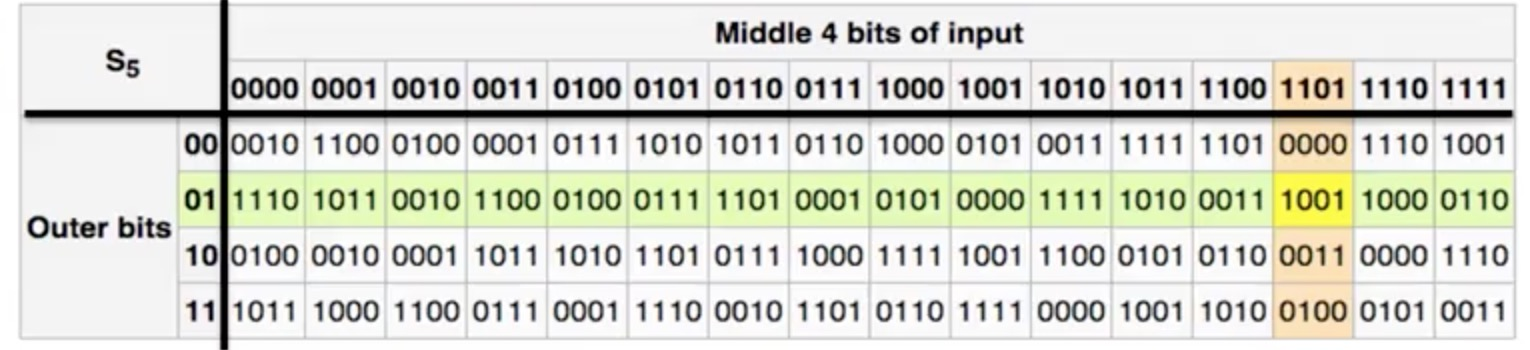
\includegraphics[width=\textwidth]{sboxeg.jpg}
\caption{An Example of $S$ Box}\label{sboxeg}
\end{figure}

The choice of these functions is subtle. For example, linear functions 
\[S_i(\vec{x})=A_i\cdot\vec{x}\pmod 2\]
with $A_i$ being a $4\times 6$ matrix are bad choices. One example could be 
\[\begin{pmatrix}
0 & 1 & 1 & 0 & 0 & 0 \\
1 & 0 & 0 & 1 & 1 & 0 \\
1 & 0 & 0 & 0 & 0 & 1 \\
0 & 1 & 1 & 0 & 0 & 1
\end{pmatrix}\cdot\begin{pmatrix}
x_1\\
x_2\\
x_3\\
x_4\\
x_5\\
x_6
\end{pmatrix} \pmod 2=\begin{pmatrix}
x_2\oplus x_3\\
x_1\oplus x_4 \oplus x_5\\
x_1\oplus x_6\\
x_2\oplus x_3\oplus x_6
\end{pmatrix}\]
The reason is that we can then find a $64\times 832$\footnote{832 = 64 + 48 * 16} matrix $B$ such that 
\begin{align*}
DES(k,m)&=B\cdot\begin{pmatrix}m&k_1&\cdots&k_{16}\end{pmatrix}^{\mathsf{T}}\coloneqq B\cdot\begin{pmatrix}m\\\mathcal{K}\end{pmatrix}\\
&=m_{i_1}\oplus\cdots\oplus m_{i_n}\oplus \mathcal{K}_{j_1}\oplus\cdots\oplus \mathcal{K}_{j_k},
\end{align*}
i.e DES as a whole becomes linear. Then we have 
\begin{align*}
 &DES(k,m_1)\oplus DES(k,m_2)\oplus DES(k,m_3)\\
=&B\cdot\begin{pmatrix}m_1\\\mathcal{K}\end{pmatrix}\oplus B\cdot\begin{pmatrix}m_2\\\mathcal{K}\end{pmatrix}\oplus  B\cdot\begin{pmatrix}m_3\\\mathcal{K}\end{pmatrix}\\
=&B\cdot\begin{pmatrix}m_1\oplus m_2\oplus m_3\\\mathcal{K}\end{pmatrix}\\
=&DES(k,m_1\oplus m_2\oplus m_3),
\end{align*}
which is not a property that holds for a random function, and thus makes DES insecure. What's worse, all round keys can be extracted given 832 $m-c$ pairs.

It has been proven that even choosing the $S$ boxes and $P$ box at random will result in an insecure block cipher. There are a lot of rules limiting the choices in order to guarantee the security of DES.
\section{Attacks on DES}
\subsection{Exhaustive Search Attack}
The goal of an \textbf{exhaustive search attack} is to recover the key $k$ given 3 input-output pairs $m_i,c_i=E(k,m_i),i=1,2,3.$ We use ``the'' key because the following lemma convinces us of its uniqueness.
\begin{lemma}
Suppose DES is an \textbf{ideal cipher}\footnote{This is idealized, not the actual situation}, i.e. DES is a collection of $2^{56}$ random invertible functions 
\[\pi_i:\{0,1\}^{64}\rightarrow\{0,1\}^{64},i=1,\dots,2^{56}.\]
Then $\forall m,c$, 
\[Pr(\text{at most one key s.t. $c=DES(k,m)$})\geq 1-\frac{1}{256}\approx 99.5\%.\]
\end{lemma}
\begin{proof}
\begin{align*}
&Pr(\exists k'\neq k\:s.t.\:c=DES(k,m)=DES(k',m))\\
\leq&\sum\limits_{k'\in\{0,1\}^{56}}Pr(DES(k',m)=c)\\
=&2^{56}\cdot\frac{1}{2^{64}}=\frac{1}{256}
\end{align*}
\end{proof}
This fact makes it possible to find the $k$ with brute force search with only one $m-c$ pair. It is not that difficult to use modern computers to do this with a 56-bit cipher, so 56-bit DES ciphers should no longer be used. 

There are ways to enhance the security of DES. 
\subsubsection{3DES}
Let $E:K\times M\rightarrow M$ be a 56-bit DES cipher. The define a 3DES cipher $3E:K^{3}\times M\rightarrow M$ as 
\[3E((k_1,k_2,k_3),m)=E(k_1,D(k_2,E(k_3,m))).\]
3DES has the key size of $56\times 3=168$. It is safer than DES, but it is also 3 times slower. We use E-D-E instead of E-E-E in order to be able to produce DES result with $k_1=k_2=k_3$.

The reason to use 3DES instead of 2DES is that 2DES is breakable with less time than it appears to need, making it insecure. Define 
\[2E((k_1,k_2,k_3),m)=E(k_1,E(k_2,m)).\]
Given a $m-c$ pair, we have 
$E(k_1,E(k_2,m))=c$, therefore $D(k_1,c)=E(k_2,m)$, which inspires us of a new way to break the cipher, namely the meet-in-the-middle attack. 

First we calculate $E(k_i,m)$ for all $2^{56}$ possible keys and save them in a table. Then we sort the table according to the value of $E(k_i,m)$. Finally for each possible $k_i$, we calculate $D(k_i,c)$ and search for it in the table. Building and sorting the table takes $2^{56}\log(2^{56})$ time. Searching for all the decryptions takes another $2^{56}\log(2^{56})$ time. In total the time consumption is smaller than $2^{63}\ll 2^{112}$, making 2DES insecure.

The same strategy can be used to break 3DES in $2^{118}$ time:
\[2^{56}\log(2^{56})+2^{56\times 2}\log(2^{56})=2^{118}.\]
\subsubsection{DESX}
Define DESX cipher $EX:K^{3}\times M\rightarrow M$ as 
\[EX((k_1,k_2,k_3),m)=k_1\oplus E(k_2,k_3\oplus m).\]
It has a key length of 64+56+64=184. A meet-in-the-middle attack takes $2^{120}$ time: using $k_1\oplus c=E(k_2,k_3\oplus m)$, the time consumption is 
\[2^{56+64}\log(2^{56+64})+2^{64}\log(2^{56+64})=2^{120}.\]

Nonetheless, if only one XOR is used, i.e. $k_1$ or $k_3$ is not used, the cipher will be no securer than DES.
\subsection{Side Channel Attacks}
An attacker can obtain the key by precisely measuring the time or power consumption of encryption/decryption. If the cipher is run in one of the cores of a multi-core processor, an attacker can obtain the key by counting the number of cache misses in the shared cache. 
\subsection{Fault Attack}
An error in the last round can expose the secret key. Thus the correctness of the algorithm needs to be guaranteed, which serves as a strong reason for us not to attempt to implement cryptography primitives.
\subsection{Linear/Differential Attacks}
The goal is to recover the key in less than $2^{56}$ time when given many $m-c$ pairs. Suppose for random $k,m$, 
\[Pr((m[i_1]\oplus\cdots\oplus m[i_r])\oplus(c[j_1]\oplus\cdots\oplus c[j_r]) = k[l_1]\oplus\cdots\oplus k[l_r])=\frac{1}{2}+\epsilon\]
holds for some non-zero $\epsilon$, in which $m[i_1]\dots m[i_r]$ is a subset of the message bits, $c[j_1]\dots c[j_r]$ is a subset of the cipher text bits, and $k[l_1]\dots k[l_r]$ is a subset of the key bits, then we have the following theorem.
\begin{theorem}
Given $\frac{1}{\epsilon^2}$ random $m-c$ pairs, then we have
\[k[l_1]\oplus\cdots\oplus k[l_r]=mode((m[i_1]\oplus\cdots\oplus m[i_r])\oplus(c[j_1]\oplus\cdots\oplus c[j_r]))\]
with a probability $\geq 97.7\%$.
\end{theorem}
Mode is the statistical mode: element with maximum frequency. 

For DES, we have $\epsilon=\frac{1}{2^{21}}$. With $2^{42}$ $m-c$ pairs we can find 14 key bits in time $2^{42}$. Then we can do a brute force search for the remaining bits in $2^{42}$ time, thus the overall attack time is $2^{43}\ll 2^{56}$. 

This is another reason against implementing our own ciphers: a little bias of the cipher leads to an easy attack.
\subsection{Quantum Attacks}
Consider a generic problem: given $f:X\rightarrow\{0,1\}$ that is a function evaluating to 0 most of the time, try to find $x\in X$ s.t. $f(x)=1$. On a classical computer, the best generic algorithm takes $O(\lvert X\rvert)$ time. A quantum on the contrary can solve the problem in $O(\sqrt{\lvert X\rvert})$ time.

To attack a block cipher, we can use the function
\begin{equation*}
f(k)=\begin{cases}
1&if\:E(k,m)=c\\
0&otherwise
\end{cases}\end{equation*}
This means that a quantum search algorithm can find the key in $O(\sqrt{\lvert K\rvert})$ time. For DES this means $2^{28}$ time. 

\section{Advanced Encryption Standard(AES)}
AES is built as a substitution-permutation network (Figure \ref{aes_network}). In each round, the input is first XOR'ed with a round key, then goes through a substitution layer in which blocks of the state are substituted according to the substitution table, and finally goes through a permutation in which bits are permuted and shuffled around. Every step must be reversible so that the whole algorithm is reversible. The decryption process is simply all the steps taken in reverse order. Specifically, Figure \ref{aes128} shows the process of AES 128 encryption.

\begin{figure}[ht]
\centering
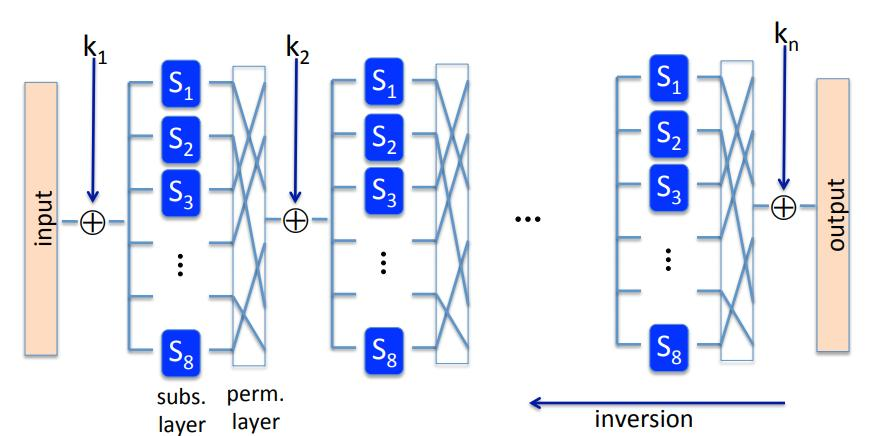
\includegraphics[width=\textwidth]{AES_network.jpg}
\caption{AES Subs-Perm Network}\label{aes_network}
\end{figure}
\begin{figure}[ht]
\centering
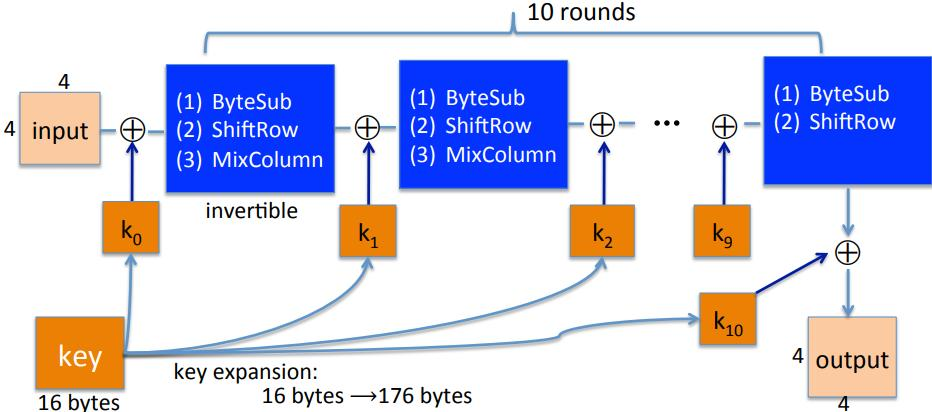
\includegraphics[width=\textwidth]{aes128.jpg}
\caption{AES 128 Schematic}\label{aes128}
\end{figure}

The 16-byte input is written as a 4$\times$4 matrix $A$. The first function $ByteSub$ is just a 1-byte S-box that maps a byte to another:
\[A[i,j]\rightarrow S[A[i,j]],\forall i,j.\]
The second function $Shiftrow$ does a cyclic shift on each row:
\begin{equation*}
\begin{bmatrix}
  S_{00} & S_{01} & S_{02} & S_{03} \\ 
  S_{10} & S_{11} & S_{12} & S_{13} \\ 
  S_{20} & S_{21} & S_{22} & S_{23} \\ 
  S_{30} & S_{31} & S_{32} & S_{33} \\ 
\end{bmatrix}\Rightarrow
\begin{bmatrix}
  S_{00} & S_{01} & S_{02} & S_{03} \\ 
  S_{11} & S_{12} & S_{13} & S_{10} \\ 
  S_{22} & S_{23} & S_{20} & S_{21} \\ 
  S_{33} & S_{30} & S_{31} & S_{32} \\ 
\end{bmatrix}.
\end{equation*}
The third function $MixColumn$ applies a linear function on each column. All 3 steps are easily computable, allowing AES to be implemented with no pre-computation (thus small code size). There is a tradeoff between code size and performance: the smaller the code size, the slower the implementation is. The javascript AES lib makes use of this fact to accelerate both code transmission through web and local computation in the browser: code with no pre-computation is transmitted from server to the browser, and pre-compute tables are computed prior to encryption.

Two types of attacks are known to exist for AES: the best key recovery attack on AES-128 (4 times faster than brute-force search, $2^{126}$) and the related key attack on AES-256 (much faster than brute-force search, $2^{99}$). 
\section{Block Ciphers from PRGs}
Let $G:K\rightarrow K^2(G(k)=G(k)[0]\parallel G(k)[1]$) be a PRG, and define a 1-bit PRF $F:K\times\{0,1\}\rightarrow K$ as 
\[F(k,x)=G(k)[x], x\in\{0,1\}.\]
Then obviously we have
\begin{theorem}
If $G$ is a secure PRG, then $F$ is a secure PRF.
\end{theorem}
\begin{figure}[ht]
\centering
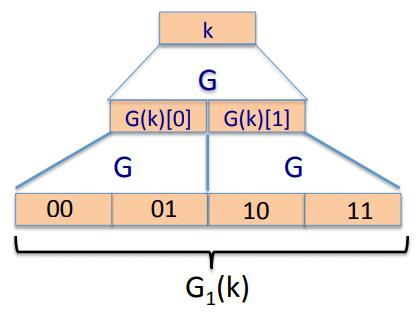
\includegraphics[width=0.5\textwidth]{prg2prf_g1.jpg}
\caption{PRG to PRF on $\{0,1\}^2$}\label{prg2prf_g1}
\end{figure}
$G,F$ can be extended to get $G_1:K\rightarrow K^4, F_1:K\times\{0,1\}^2\rightarrow K$, as shown in Figure \ref{prg2prf_g1}. The security of $G_1$ can be proved according to the security of $G$.
\begin{align*}
G_1(k)&=G(G(k)[0])\parallel G(G(k)[1])\\
F_1(k, x)&=G_1(k)[x]
\end{align*}

We can extend more and more to obtain a secure PRF(the GGM PRF) on $K\times\{0,1\}^n$.
\begin{align*}
\begin{cases}
  k_1&=G(k)[x_0]\\
k_2&=G(k1)[x_1]\\
&\cdots\\
k_n&=G(k_{n-1})[x_{n-1}]\\
\end{cases}\\
F(k,x_0x_1\cdots x_{n-1})=k_n\\
\end{align*}
According to Theorem \ref{lubyrackoff}, a $2n$ bit PRP can be obtained from the PRF, thus a block cipher can be defined. This secure PRF and the block cipher it defines is not used in practice because it is too slow ($n$ times slower than the original PRG).
\begin{lemma}
\textbf{PRF Switching Lemma}
Let $E$ be a PRP over $(K,X)$, then for any $q$-query adversary $A$,
\[\left\lvert Adv_{PRP}[A,E]-Adv_{PRF}[A,E]\right\rvert<\frac{q^2}{2|X|},\]
i.e. as long as $|X|$ is large enough, a secure PRP is also a secure PRF.
\end{lemma}
\section{Using Block Ciphers: One-Time Keys}
\begin{itemize}
\item adversary's ability: sees only one cipher text (one-time key)
\item adversary's goal: learn info about plain text from cipher text
\end{itemize}

\subsection{Incorrect Use: Electronic Code Book}
A common incorrect use of a block cipher is \textbf{electronic code book}: divide the message into blocks and encrypt each block independently ($E(m_i) = c_i$). Obviously $c_1 = c_2$ when $m_1=m_2$. It is not semantically secure: $m_0$ = \texttt{HelloHello} and $m_1$ = \texttt{HelloWorld} would be enough to tell it from a random function (suppose block size = 5).
\subsection{Deterministic Counter Mode}
Deterministic counter mode generates a stream cipher from a block cipher (i.e. a PRF) $F$.
\begin{figure}[ht]
  \centering
  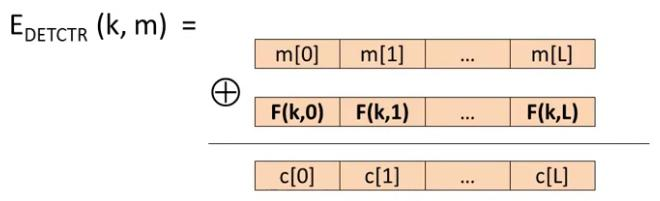
\includegraphics[width=\textwidth]{detctr.jpg}
  \caption{Deterministic Counter Mode}\label{detctr}
\end{figure}

\section{Using Block Ciphers: Many-Time Keys}
\begin{itemize}
  \item adversary's ability: \textbf{chosen-plaintext attack (CPA)}. Can obtain the encryption of arbitrary messages of his choice (by providing the same message twice in a semantic security challenge)
  \item adversary's goal: break semantic security
\end{itemize}

If a cipher always outputs the same cipher text for a given message $m$, then it is insecure under CPA. In a semantic security challenge, the adversary can do as such:
\begin{itemize}
  \item Round 1: provide $m, m$ to obtain $c$ the ciphertext of $m$
  \item Round 2: provide $m, m_1$, if obtain $c$: output 0; otherwise output 1
\end{itemize}
\subsection{CPA Security}
\subsubsection{Randomized Encryption}
$E(k,m)$ is a randomized algorithm. Encrypting the same msg twice gives different cipher texts. The cipher text must be longer than the plain text. Roughly speaking, length of CT = length of PT + \#random bits. If the PT is quite long, the overhead is negligible. But if PT itself is short, the overhead would become a problem.
\subsubsection{Nonce-Based Encryption}
\begin{itemize}
\item Encryption: $E(k, m, n) = c$
\item Decryption: $D(k, c, n) = m$
\end{itemize}
Nonce $n$ is a value that changes from value to value so that the pair $(k,n)$ is never used more than once. It does not have to be random.

The nonce can be a counter (packet number). It can be used when the encryptor keeps a state from msg to msg, and it does not have to be sent together with the CT if the decryptor keeps the same state. It can also be chosen at random from a large enough space $N$, in which the encryptor does not have to maintain any state.

The system should be secure when the nonce is chosen by the adversary. But the adversary has  to choose a different nonce each time.
\subsection{Cipher Block Chain}
Let $E,D$ be a PRP. Choose a random $IV\in X$ (IV = initialization vector) with the same length as a cipher block, and do the following:
\[c[0]=E(k, IV\oplus m[0])\]
\[c[i]=E(k, c[i-1]\oplus m[i]), i\ge 1\]
The CT is one block longer than the PT because it includes the IV. To decrypt the CT, we have
\[m[0]=D(k, c[0])\oplus IV\]
\[m(i)=D(k, c[i])\oplus c[i-1], i\ge 1\]
\begin{theorem}\textbf{CBC Theorem}
For any $L>0$, if $E$ is a secure PRP over $(K,X)$, then $E_{CBC}$ is semantically secure cipher under CPA over $(K, X^L, X^{L+1})$. In particular, for a $q-$query adversary $A$ attacking $E_{CBC}$, there exists a PRP adverdary $B$ such that
\[Adv_{CPA}[A, E_{CBC}]\le Adv_{PRP}(B, E)+\frac{2q^2L^2}{|X|}\]
\end{theorem}
The theorem means that CBC is only secure when $q^2L^2\ll |X|$. $q$ is number of messages encrypted with $k$, and $L$ is max length of the message (in blocks). 

It is crucial that the IV be random for each message. If the IV can be predicted, CBC is not CPA secure. If a non-random nonce is used instead of a random IV, it has to be encrypted with a distinct key $k_1$ before being used in place of the IV.
\subsection{Randomized Counter Mode}
\begin{figure}[ht]
  \centering
  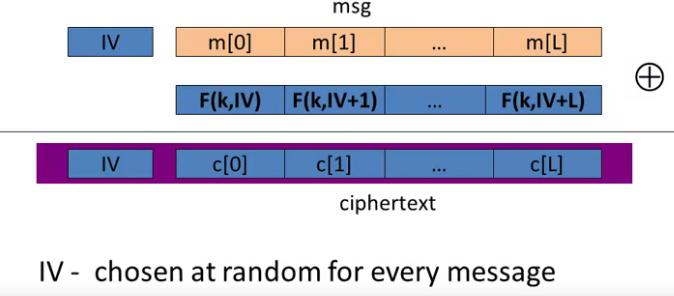
\includegraphics[width=\textwidth]{randomctrmode.jpg}
  \caption{Randomized Counter Mode}\label{randomctrmode}
\end{figure}

Randomized counter mode is superior to CBC in every aspect:

\begin{figure}[ht]
  \centering
  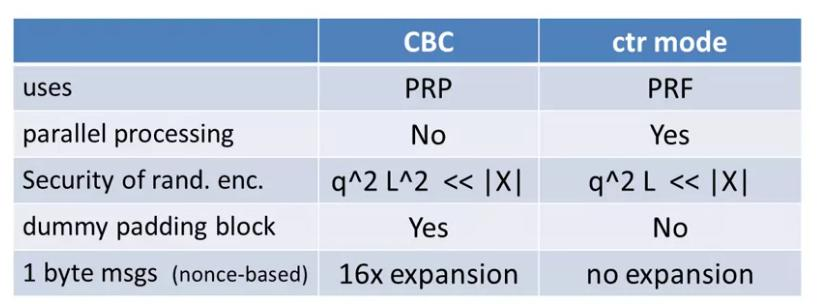
\includegraphics[width=\textwidth]{ctrcbccomp.jpg}
  \caption{Randomized Counter Mode v.s. CBC}\label{ctrcbccomp}
\end{figure}

\ifx\PREAMBLE\undefined
\end{document}
\fi